\documentclass[a4paper, 14pt]{extarticle}

% Поля
%--------------------------------------
\usepackage{geometry}
\geometry{a4paper,tmargin=2cm,bmargin=2cm,lmargin=3cm,rmargin=1cm}
%--------------------------------------


%Russian-specific packages
%--------------------------------------
\usepackage[T2A]{fontenc}
\usepackage[utf8]{inputenc} 
\usepackage[english, main=russian]{babel}
%--------------------------------------

\usepackage{textcomp}

% Красная строка
%--------------------------------------
\usepackage{indentfirst}               
%--------------------------------------             


%Graphics
%--------------------------------------
\usepackage{graphicx}
\graphicspath{ {./images/} }
\usepackage{wrapfig}
%--------------------------------------

% Полуторный интервал
%--------------------------------------
\linespread{1.3}                    
%--------------------------------------

%Выравнивание и переносы
%--------------------------------------
% Избавляемся от переполнений
\sloppy
% Запрещаем разрыв страницы после первой строки абзаца
\clubpenalty=10000
% Запрещаем разрыв страницы после последней строки абзаца
\widowpenalty=10000
%--------------------------------------

%Списки
\usepackage{enumitem}

%Подписи
\usepackage{caption} 

%Гиперссылки
\usepackage{hyperref}

\hypersetup {
	unicode=true
}

%Рисунки
%--------------------------------------
\DeclareCaptionLabelSeparator*{emdash}{~--- }
\captionsetup[figure]{labelsep=emdash,font=onehalfspacing,position=bottom}
%--------------------------------------

\usepackage{tempora}
\usepackage{amsmath}
\usepackage{color}
\usepackage{listings}
\lstset{
  belowcaptionskip=1\baselineskip,
  breaklines=true,
  frame=L,
  xleftmargin=\parindent,
  language=Python,
  showstringspaces=false,
  basicstyle=\footnotesize\ttfamily,
  keywordstyle=\bfseries\color{blue},
  commentstyle=\itshape\color{purple},
  identifierstyle=\color{black},
  stringstyle=\color{red},
}

%--------------------------------------
%			НАЧАЛО ДОКУМЕНТА
%--------------------------------------

\begin{document}

%--------------------------------------
%			ТИТУЛЬНЫЙ ЛИСТ
%--------------------------------------
\begin{titlepage}
\thispagestyle{empty}
\newpage


%Шапка титульного листа
%--------------------------------------
\vspace*{-60pt}
\hspace{-65pt}
\begin{minipage}{0.3\textwidth}
\hspace*{-20pt}\centering

\includegraphics[width=\textwidth]{emblem}
\end{minipage}
\begin{minipage}{0.67\textwidth}\small \textbf{
\vspace*{-0.7ex}
\hspace*{-6pt}\centerline{Министерство науки и высшего образования Российской Федерации}
\vspace*{-0.7ex}
\centerline{Федеральное государственное бюджетное образовательное учреждение }
\vspace*{-0.7ex}
\centerline{высшего образования}
\vspace*{-0.7ex}
\centerline{<<Московский государственный технический университет}
\vspace*{-0.7ex}
\centerline{имени Н.Э. Баумана}
\vspace*{-0.7ex}
\centerline{(национальный исследовательский университет)>>}
\vspace*{-0.7ex}
\centerline{(МГТУ им. Н.Э. Баумана)}}
\end{minipage}
%--------------------------------------

%Полосы
%--------------------------------------
\vspace{-25pt}
\hspace{-35pt}\rule{\textwidth}{2.3pt}

\vspace*{-20.3pt}
\hspace{-35pt}\rule{\textwidth}{0.4pt}
%--------------------------------------

\vspace{1.5ex}
\hspace{-35pt} \noindent \small ФАКУЛЬТЕТ\hspace{80pt} <<Информатика и системы управления>>

\vspace*{-16pt}
\hspace{47pt}\rule{0.83\textwidth}{0.4pt}

\vspace{0.5ex}
\hspace{-35pt} \noindent \small КАФЕДРА\hspace{50pt} <<Прикладная математика и информатика>>

\vspace*{-16pt}
\hspace{30pt}\rule{0.866\textwidth}{0.4pt}
  
\vspace{11em}

\begin{center}
\Large {\bf Лабораторная работа № 5} \\ 
\large {\bf по курсу <<Языки и методы программирования>>} \\ 
\large <<Монады в языке Java>>
\end{center}\normalsize

\vspace{8em}


\begin{flushright}
  {Студент группы ИУ9-21Б Хромов М.А.\hspace*{15pt} \\
  \vspace{2ex}
  Преподаватель Посевин Д. П.\hspace*{15pt}}
\end{flushright}

\bigskip

\vfill
 

\begin{center}
\textsl{Москва 2025}
\end{center}
\end{titlepage}
%--------------------------------------
%		КОНЕЦ ТИТУЛЬНОГО ЛИСТА
%--------------------------------------

\renewcommand{\ttdefault}{pcr}

\setlength{\tabcolsep}{3pt}
\newpage
\section{Цель}\label{Sect::task}
\par
Приобретение навыков использования монад Optional и Stream в программах на языке Java. 


\section{Задание}\label{Sect::task}
\par
Во время выполнения лабораторной работы требуется разработать на языке Java один из классов, перечисленных в таблице, которая приведена ниже.
\par
В каждом классе нужно реализовать по крайней мере два метода: первый метод должен возвращать Stream, а второй – Optional. Операции, выполняемые каждым методом, указаны в вариантах задания. 
\par
В методе main вспомогательного класса Test нужно продемонстрировать работоспособность разработанного класса, осуществив группировку содержимого потока, возвращаемого первым методом, с помощью группирующего коллектора. 
\par
В исходном коде (включая класс Test) запрещено использовать циклы и рекурсию.  

\section{Индивидуальный вариант}
\par
Вариант 28 + Вариант 26
\par 
Множество квадратных трёхчленов вида a·x2 + b·x + c, в которых a != 0, с операциями: 
1. порождение потока сумм корней соответствующих квадратных уравнений (вспомнить теорему Виета), имеющих действительные решения; 
2. поиск трёхчлена с максимальным произведением корней. 
Проверить работу первой операции нужно путём подсчёта количества отрицательных и неотрицательных сумм. 

\par
Таблица, отображающая фамилии, имена и отчества сотрудников работающих на аутсорсе в стоимость их нормочаса и времени, которое эти сотрудники могут тратить на выполнение работы в неделю выраженное в часах, с операциями: 

1. порождение потока фамилий, имен и отчеств сотрудников работающих на аутсорсе, стоимость нормочаса которых превышает указанную сумму денег; 
2. поиск сотрудника, у которого количество времен, которое он может тратить на выполнение работы превышает суммарное количество времени, которое могут тратить на выполнение работы все остальные сотрудники (самый свободный аутсорсер). 

Проверить работу первой операции нужно путём группировки фамилий, имен и отчеств по первой букве фамилии. 


\section {Практическая реализация}
Исходный код программы представлен в листингах~\ref{lst:code1}--~\ref{lst:code4}.
\begin{figure}[!htb]
\begin{lstlisting}[language={},caption={Основной класс для варинта 28 },label={lst:code1}]
import java.util.*;
import java.util.stream.Collectors;
import java.util.stream.Stream;
class Outsourcer {
    String surname;
    String name;
    String patronymic;
    int hourlyRate;
    int weeklyHours;
    Outsourcer(String surname, String name, String patronymic, int hourlyRate, int weeklyHours) {
        this.surname = surname;
        this.name = name;
        this.patronymic = patronymic;
        this.hourlyRate = hourlyRate;
        this.weeklyHours = weeklyHours;
    }
    public String getFullName() {
        return surname + " " + name + " " + patronymic;
    }
    public int getHourlyRate() {
        return hourlyRate;
    }

    public int getWeeklyHours() {
        return weeklyHours;
    }

    public String getSurname() {
        return surname;
    }

}
class OutsourcerTable {
    private final List<Outsourcer> outsourcers = new ArrayList<>();
    public void add(Outsourcer o) {
        outsourcers.add(o);
    }

    public void add(String surname, String name, String patronymic, int hourlyRate, int weeklyHours) {
        outsourcers.add(new Outsourcer(surname, name, patronymic, hourlyRate, weeklyHours));
    }
    public Stream<String> expensiveOutsourcers(int rateThreshold) {
        return outsourcers.stream()
                .filter(o -> o.getHourlyRate() > rateThreshold)
                .map(Outsourcer::getFullName);
    }
    public Optional<Outsourcer> mostAvailableOutsourcer() {
        int totalHours = outsourcers.stream()
                .mapToInt(Outsourcer::getWeeklyHours)
                .sum();
        return outsourcers.stream()
                .filter(o -> o.getWeeklyHours() > totalHours - o.getWeeklyHours())
                .findFirst();
    }
}



\end{lstlisting}
\end{figure}
\newpage
\begin{figure}[!htb]
\begin{lstlisting}[language={},caption={Основной класс для варианта 26 },label={lst:code2}]
import java.util.*;
import java.util.stream.*;

public class QuadraticPolynomial {
    private final double a;
    private final double b;
    private final double c;

    public QuadraticPolynomial(double a, double b, double c) {
        if (a == 0) {
            throw new IllegalArgumentException("'a' не должен быть равен нулю");
        }
        this.a = a;
        this.b = b;
        this.c = c;
    }

    public static Stream<Double> streamOfRootSums(List<QuadraticPolynomial> polynomials) {
        return polynomials.stream()
                .filter(p -> p.hasRealRoots())
                .map(p -> -p.b / p.a);
    }

    private boolean hasRealRoots() {
        return getDiscriminant() >= 0;
    }

    private double getDiscriminant() {
        return b * b - 4 * a * c;
    }

    public static Optional<QuadraticPolynomial> maxProductOfRoots(List<QuadraticPolynomial> polynomials) {
        return polynomials.stream()
                .filter(p -> p.hasRealRoots())
                .max(Comparator.comparingDouble(p -> p.c / p.a));
    }

    public double getA() { return a; }
    public double getB() { return b; }
    public double getC() { return c; }
}



\end{lstlisting}
\end{figure}
\newpage
\begin{figure}[!htb]
\begin{lstlisting}[language={},caption={Тестовый класс для варинта 28 },label={lst:code3}]
import java.util.List;
import java.util.Map;
import java.util.stream.Collectors;

public class Test {
    public static void main(String[] args) {
        OutsourcerTable table = new OutsourcerTable();
        table.add("Иванов", "Иван", "Иванович", 1500, 20);
        table.add("Петров", "Петр", "Петрович", 1200, 15);
        table.add("Волков", "Константин", "Аутсорсович", 2000, 50);
        table.add("Алексеев", "Алексей", "Алексеевич", 1800, 5);


        Map<Character, List<String>> grouped = table.expensiveOutsourcers(1300)
                .collect(Collectors.groupingBy(name -> name.charAt(0)));

        grouped.forEach((initial, names) ->
                System.out.println(initial + ": " + names)
        );

        table.mostAvailableOutsourcer().ifPresent(o ->
                System.out.println("Самый свободный аутсорсер: " + o.getFullName())
        );
    }
}


\end{lstlisting}
\end{figure}
\newpage
\begin{figure}[!htb]
\begin{lstlisting}[language={},caption={Тестовый класс для варинта 26},label={lst:code4}]
import java.util.Arrays;
import java.util.List;
import java.util.Map;
import java.util.Optional;
import java.util.stream.Collectors;
import java.util.stream.Stream;

class Test {
    public static void main(String[] args) {
        List<QuadraticPolynomial> polynomials = Arrays.asList(
                new QuadraticPolynomial(1, -3, 2),  // x^2 - 3x + 2
                new QuadraticPolynomial(1, -2, 1),  // x^2 - 2x + 1
                new QuadraticPolynomial(1, 2, 1),   // x^2 + 2x + 1
                new QuadraticPolynomial(2, -4, 2)   // 2x^2 - 4x + 2
        );

        Stream<Double> rootSums = QuadraticPolynomial.streamOfRootSums(polynomials);
        Map<Boolean, Long> countBySign = rootSums
                .collect(Collectors.partitioningBy(sum -> sum < 0, Collectors.counting()));

        System.out.println("Количество отрицательных сумм корней: " + countBySign.get(true));
        System.out.println("Количество неотрицательных сумм корней: " + countBySign.get(false));

        Optional<QuadraticPolynomial> maxProductPolynomial = QuadraticPolynomial.maxProductOfRoots(polynomials);

        maxProductPolynomial.ifPresent(p ->
                System.out.println("Трехчлен с максимальным произведением корней: " +
                        p.getA() + "x² + " + p.getB() + "x + " + p.getC())
        );
    }
}



\end{lstlisting}
\end{figure}
\clearpage
\newpage

\section{}
\begin{center}
    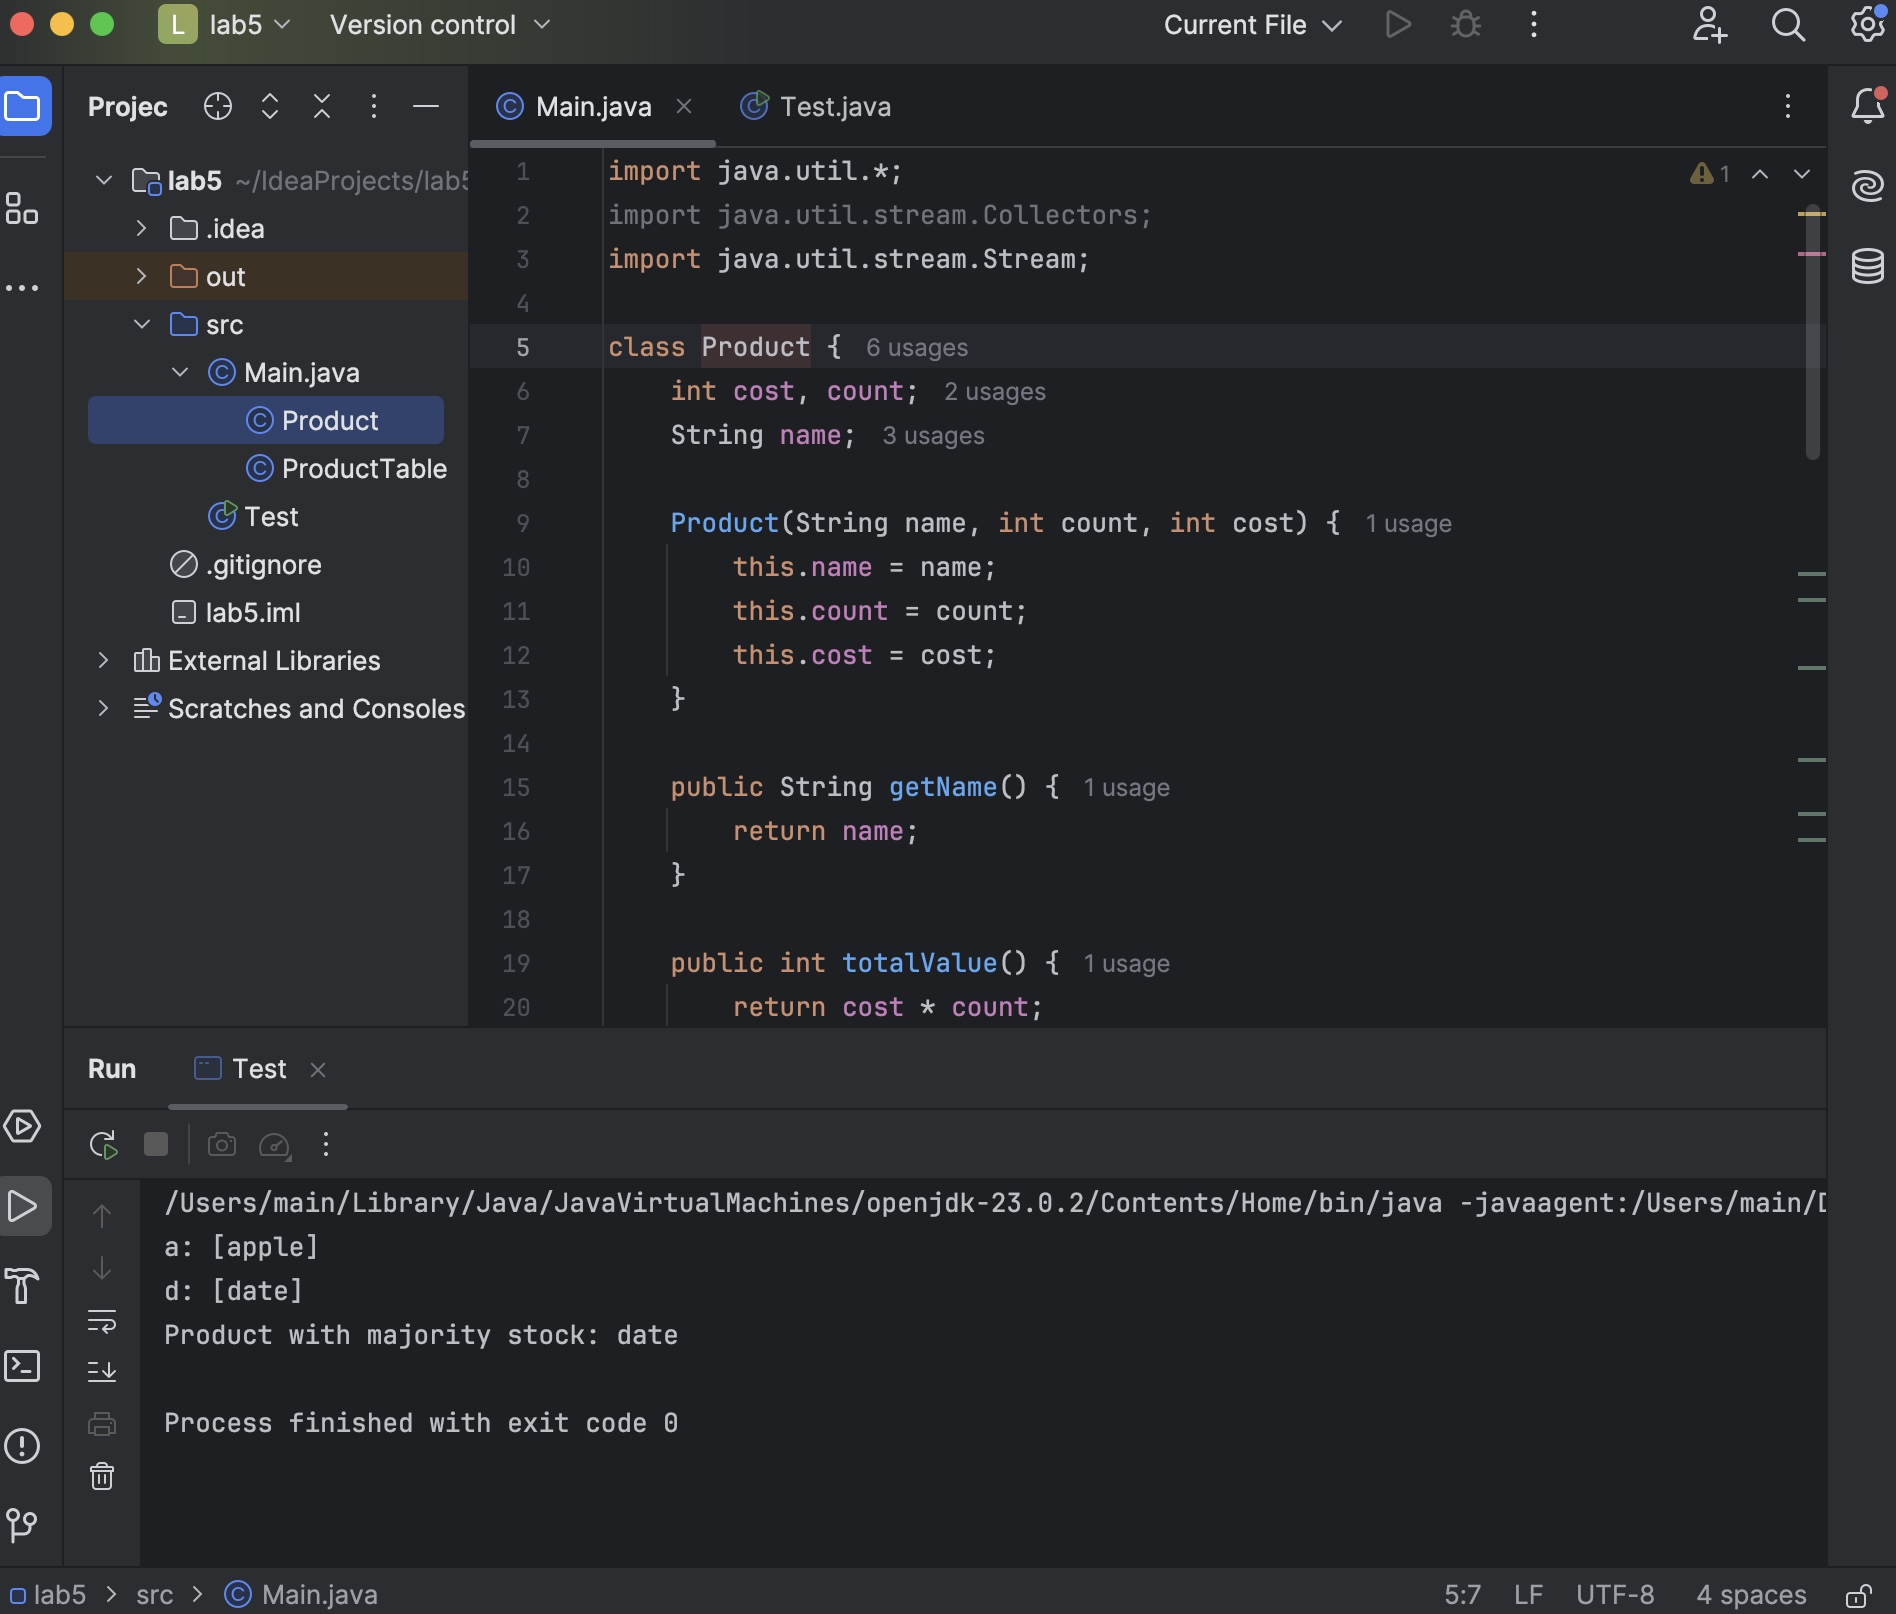
\includegraphics[width=0.8\textwidth]{фото8.jpeg}
    \captionof{figure}{Запуск тестовой программы}
\end{center}
\section{}
\begin{center}
    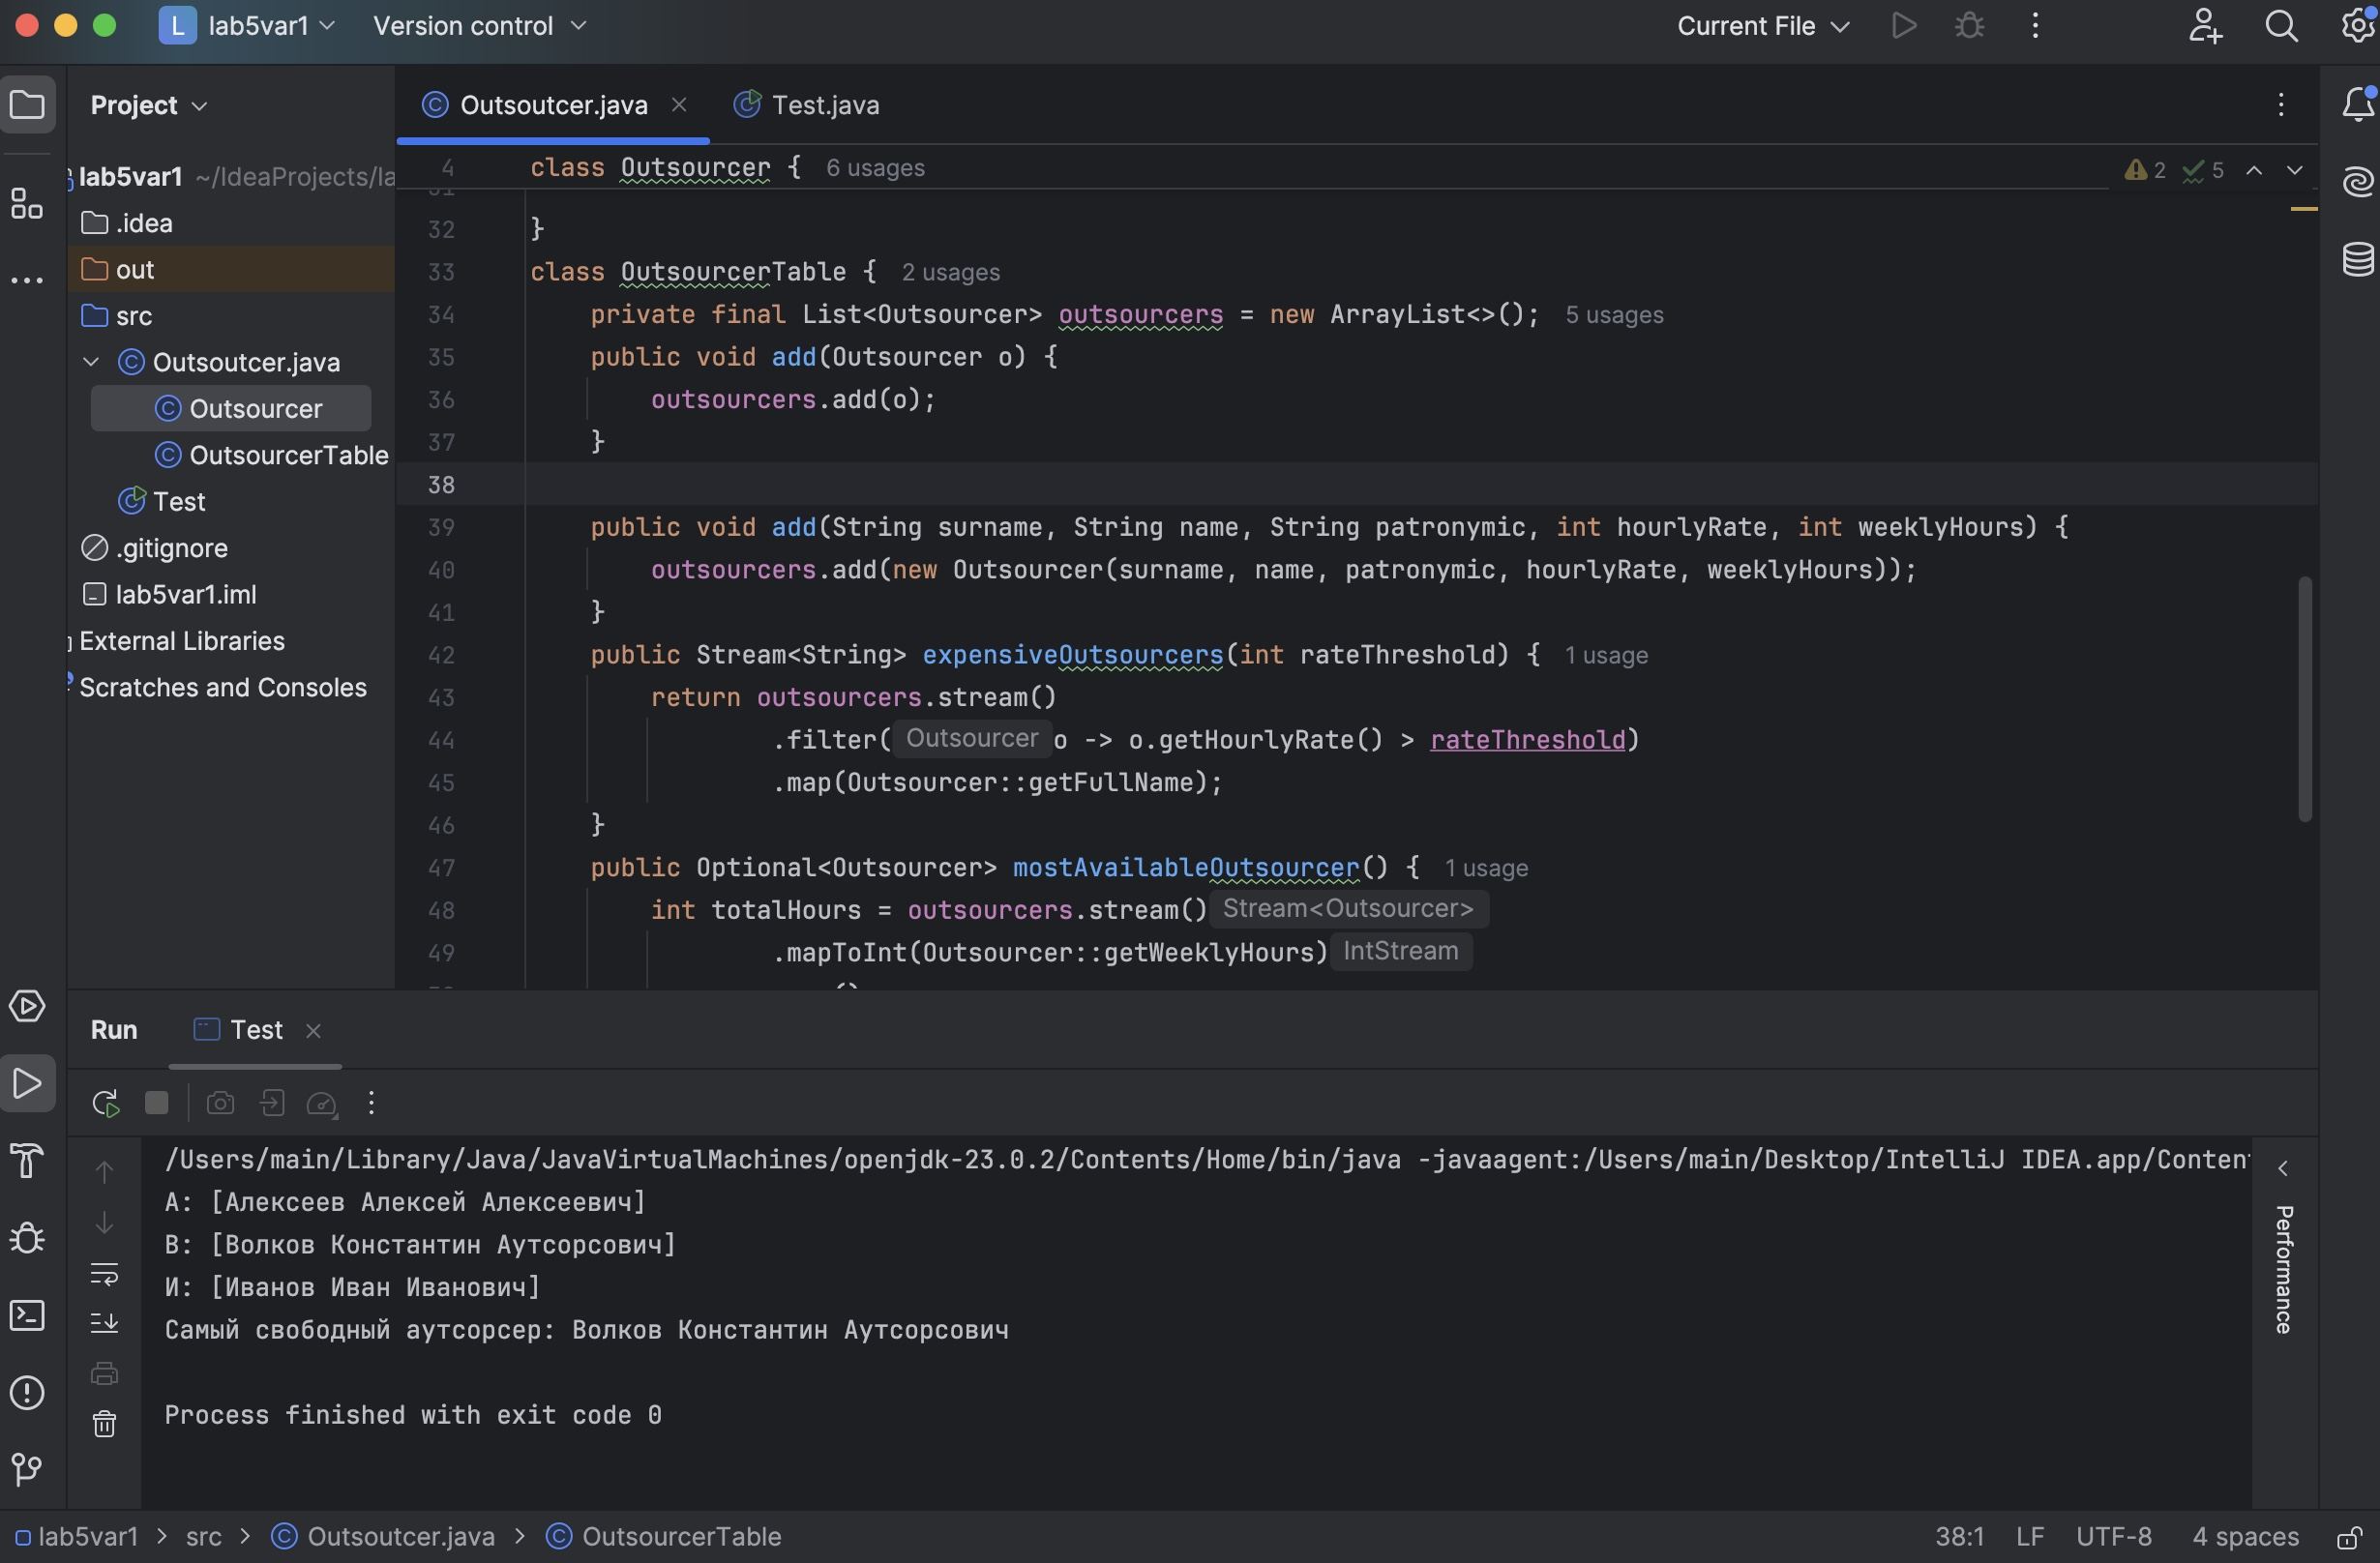
\includegraphics[width=0.8\textwidth]{фото9.jpeg}
    \captionof{figure}{Запуск программы(вар28)}
\end{center}


\section{}
\begin{center}
    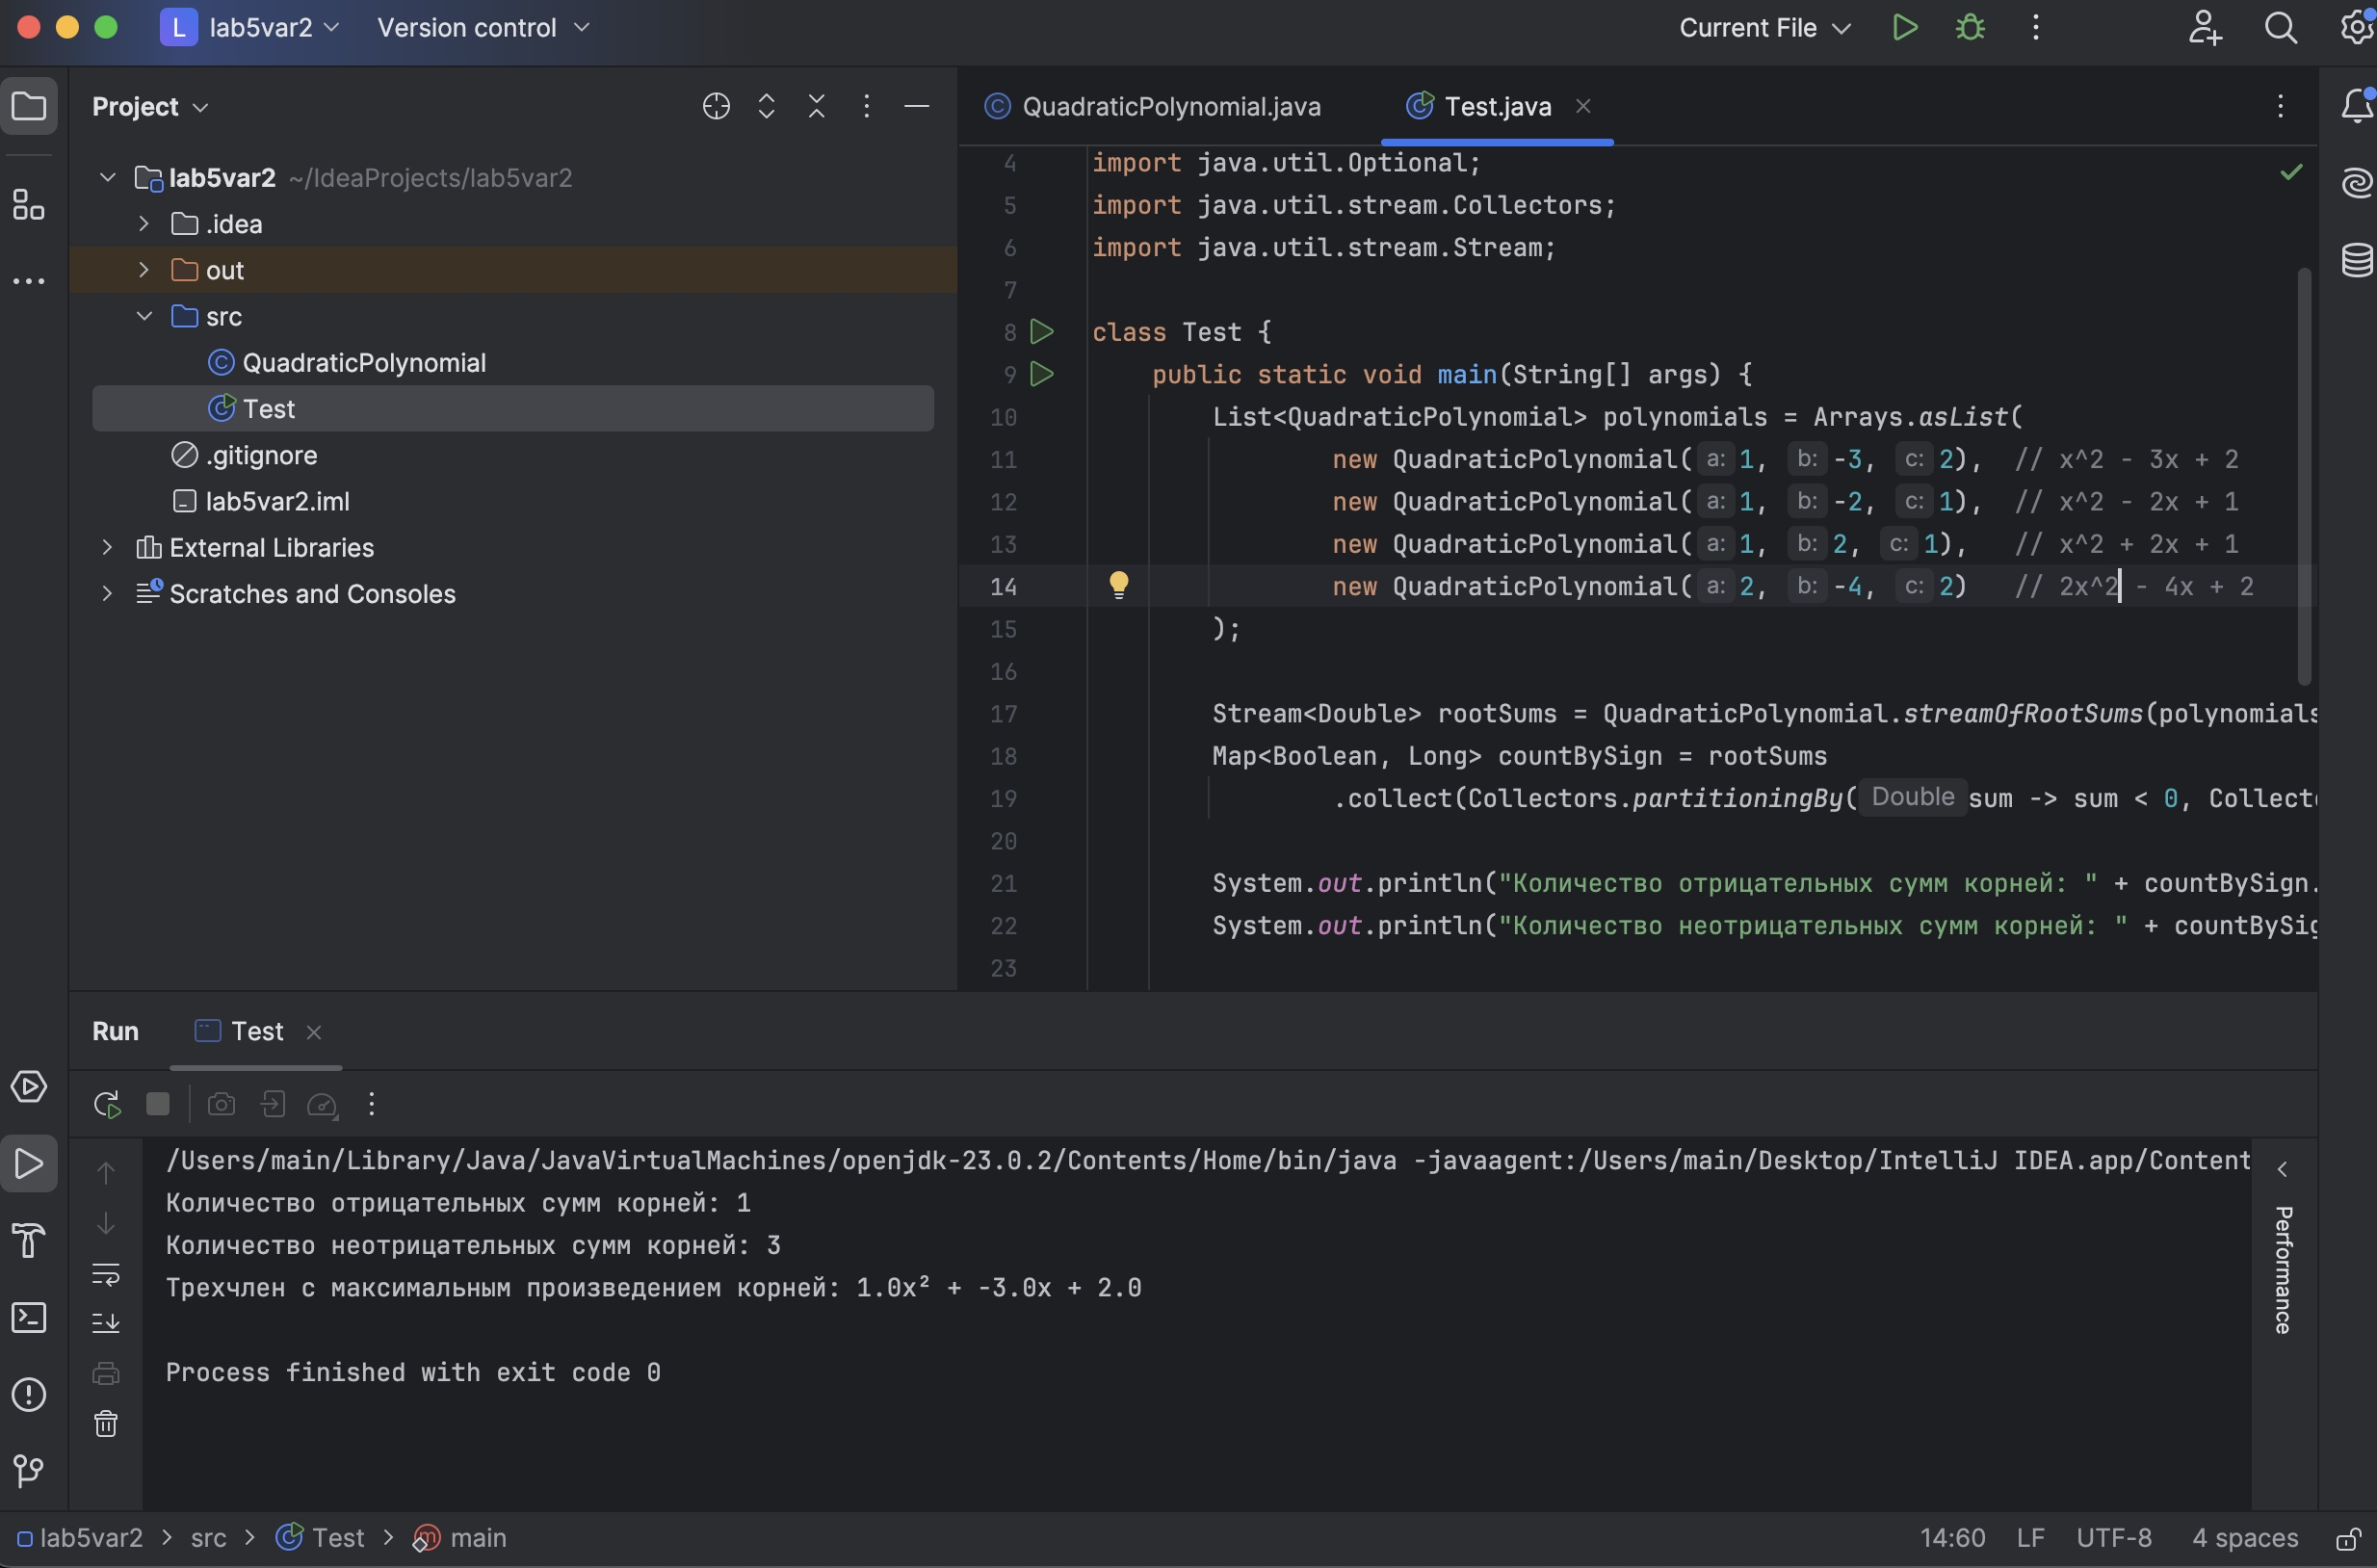
\includegraphics[width=0.8\textwidth]{фото10.jpeg}
    \captionof{figure}{Запуск программы(вар28)}
\end{center}

\section{Вывод}
В ходе выполнения лабораторной работы были приобретены навыки работы с монадами Optional и Stream в Java. Были реализованы методы, возвращающие Stream для обработки коллекций данных и Optional для безопасного поиска элементов.

На примере работы с таблицей сотрудников-аутсорсеров продемонстрированы:

Фильтрация и группировка данных с помощью Stream API.

Использование Optional для безопасного извлечения результата.

Применение группирующих коллекторов для анализа данных.

Работа показала эффективность использования Stream API для обработки данных без применения циклов и рекурсии, а также удобство Optional для обработки возможных отсутствующих значений.

\end{document}